\documentclass[dvipdfmx]{jsarticle}
\setcounter{section}{2}
\setcounter{subsection}{6}
\usepackage{xr}
\externaldocument{2.1.2}
\externaldocument{2.2.1}
\externaldocument{2.2.2}
\externaldocument{2.2.4}
\externaldocument{2.2.5}
\externaldocument{2.2.6}
\usepackage{amsmath,amsfonts,amssymb,array,comment,mathtools,url,docmute}
\usepackage{longtable,booktabs,dcolumn,tabularx,mathtools,multirow,colortbl,xcolor}
\usepackage[dvipdfmx]{graphics}
\usepackage{bmpsize}
\usepackage{amsthm}
\usepackage{enumitem}
\setlistdepth{20}
\renewlist{itemize}{itemize}{20}
\setlist[itemize]{label=•}
\renewlist{enumerate}{enumerate}{20}
\setlist[enumerate]{label=\arabic*.}
\setcounter{MaxMatrixCols}{20}
\setcounter{tocdepth}{3}
\newcommand{\rotin}{\text{\rotatebox[origin=c]{90}{$\in $}}}
\newcommand{\amap}[6]{\text{\raisebox{-0.7cm}{\begin{tikzpicture} 
  \node (a) at (0, 1) {$\textstyle{#2}$};
  \node (b) at (#6, 1) {$\textstyle{#3}$};
  \node (c) at (0, 0) {$\textstyle{#4}$};
  \node (d) at (#6, 0) {$\textstyle{#5}$};
  \node (x) at (0, 0.5) {$\rotin $};
  \node (x) at (#6, 0.5) {$\rotin $};
  \draw[->] (a) to node[xshift=0pt, yshift=7pt] {$\textstyle{\scriptstyle{#1}}$} (b);
  \draw[|->] (c) to node[xshift=0pt, yshift=7pt] {$\textstyle{\scriptstyle{#1}}$} (d);
\end{tikzpicture}}}}
\newcommand{\twomaps}[9]{\text{\raisebox{-0.7cm}{\begin{tikzpicture} 
  \node (a) at (0, 1) {$\textstyle{#3}$};
  \node (b) at (#9, 1) {$\textstyle{#4}$};
  \node (c) at (#9+#9, 1) {$\textstyle{#5}$};
  \node (d) at (0, 0) {$\textstyle{#6}$};
  \node (e) at (#9, 0) {$\textstyle{#7}$};
  \node (f) at (#9+#9, 0) {$\textstyle{#8}$};
  \node (x) at (0, 0.5) {$\rotin $};
  \node (x) at (#9, 0.5) {$\rotin $};
  \node (x) at (#9+#9, 0.5) {$\rotin $};
  \draw[->] (a) to node[xshift=0pt, yshift=7pt] {$\textstyle{\scriptstyle{#1}}$} (b);
  \draw[|->] (d) to node[xshift=0pt, yshift=7pt] {$\textstyle{\scriptstyle{#2}}$} (e);
  \draw[->] (b) to node[xshift=0pt, yshift=7pt] {$\textstyle{\scriptstyle{#1}}$} (c);
  \draw[|->] (e) to node[xshift=0pt, yshift=7pt] {$\textstyle{\scriptstyle{#2}}$} (f);
\end{tikzpicture}}}}
\renewcommand{\thesection}{第\arabic{section}部}
\renewcommand{\thesubsection}{\arabic{section}.\arabic{subsection}}
\renewcommand{\thesubsubsection}{\arabic{section}.\arabic{subsection}.\arabic{subsubsection}}
\everymath{\displaystyle}
\allowdisplaybreaks[4]
\usepackage{vtable}
\theoremstyle{definition}
\newtheorem{thm}{定理}[subsection]
\newtheorem*{thm*}{定理}
\newtheorem{dfn}{定義}[subsection]
\newtheorem*{dfn*}{定義}
\newtheorem{axs}[dfn]{公理}
\newtheorem*{axs*}{公理}
\renewcommand{\headfont}{\bfseries}
\makeatletter
  \renewcommand{\section}{%
    \@startsection{section}{1}{\z@}%
    {\Cvs}{\Cvs}%
    {\normalfont\huge\headfont\raggedright}}
\makeatother
\makeatletter
  \renewcommand{\subsection}{%
    \@startsection{subsection}{2}{\z@}%
    {0.5\Cvs}{0.5\Cvs}%
    {\normalfont\LARGE\headfont\raggedright}}
\makeatother
\makeatletter
  \renewcommand{\subsubsection}{%
    \@startsection{subsubsection}{3}{\z@}%
    {0.4\Cvs}{0.4\Cvs}%
    {\normalfont\Large\headfont\raggedright}}
\makeatother
\makeatletter
\renewenvironment{proof}[1][\proofname]{\par
  \pushQED{\qed}%
  \normalfont \topsep6\p@\@plus6\p@\relax
  \trivlist
  \item\relax
  {
  #1\@addpunct{.}}\hspace\labelsep\ignorespaces
}{%
  \popQED\endtrivlist\@endpefalse
}
\makeatother
\renewcommand{\proofname}{\textbf{証明}}
\usepackage{tikz,graphics}
\usepackage[dvipdfmx]{hyperref}
\usepackage{pxjahyper}
\hypersetup{
 setpagesize=false,
 bookmarks=true,
 bookmarksdepth=tocdepth,
 bookmarksnumbered=true,
 colorlinks=false,
 pdftitle={},
 pdfsubject={},
 pdfauthor={},
 pdfkeywords={}}
\begin{document}
%\hypertarget{jordanux5206ux89e3}{%
\subsection{Jordan分解}%\label{jordanux5206ux89e3}}
%\hypertarget{jordanux5206ux89e3-1}{%
\subsubsection{Jordan分解}%\label{jordanux5206ux89e3-1}}
\begin{thm}[Jordan分解]\label{2.2.7.1}
代数的閉体$K$上の$n$次元vector空間$V$における任意の線形写像$f:V \rightarrow V$に対し、対角化可能な線形写像$R:V \rightarrow V$と冪零変換$G:V \rightarrow V$が存在して$f = R + G$が成り立つかつ、$R \circ G = G \circ R$が成り立つ。\par
この定理をJordan分解という。
\end{thm}\par
より詳しくいえば、そのような線形写像$R$の一例として\footnote{ホントは後述するようにコレしかないんですけどね…汗}、分解定理よりその線形写像$f$の互いに異なる固有値の族$\left\{ \lambda_{i} \right\}_{i \in \varLambda_{s}}$が与えられたらば、これらの広義の固有空間たち$\widetilde{W_{f}}\left( \lambda_{i} \right)$を用いて$V = \bigoplus_{i \in \varLambda_{s}} {\widetilde{W_{f}}\left( \lambda_{i} \right)}$が成り立つので、そのvector空間$V$からその広義の固有空間$\widetilde{W_{f}}\left( \lambda_{i} \right)$への直和分解から定まる射影$P_{i}$を用いて$R = \sum_{i \in \varLambda_{s}} {\lambda_{i}P_{i}}$が成り立つ。この定理を$S + N$分解ともいう\footnote{半単純 : semi-simple、冪零 : nilpotentが語源だそうです。}。
\begin{dfn}
上記の定理における線形写像たち$R$、$G$をそれぞれその線形写像$f$の半単純部分、冪零部分という。
\end{dfn}
\begin{proof}
代数的閉体$K$上の$n$次元vector空間$V$における任意の線形写像$f:V \rightarrow V$に対し、これの固有多項式$\varPhi_{f}$が互いに異なるその体$K$の元々$\lambda_{i}$を用いて$\sum_{i \in \varLambda_{s}} n_{i} = n$として次式のように表されることができるので、そうするとき、
\begin{align*}
\varPhi_{f} = \prod_{i \in \varLambda_{s}} \left( X - \lambda_{i} \right)^{n_{i}}
\end{align*}
分解定理より$\forall i \in \varLambda_{s}$に対し、その線形写像$f$の固有値$\lambda_{i}$の広義の固有空間$\widetilde{W_{f}}\left( \lambda_{i} \right)$は$\widetilde{W_{f}}\left( \lambda_{i} \right) = \ker\left( \lambda_{i}I_{V} - f \right)^{n_{i}}$を満たす。このとき、この広義の固有空間$\widetilde{W_{f}}\left( \lambda_{i} \right)$における線形写像$\lambda_{i}I_{V} - f$は冪零変換であり、その広義の固有空間$\widetilde{W_{f}}\left( \lambda_{i} \right)$においてそれらの線形写像たち$\lambda_{i}I_{V}$、$f - \lambda_{i}I_{V}$と一致するような線形写像たち$R$、$G$が与えられたらば、$\forall\mathbf{v} \in V$に対し、分解定理より$V = \bigoplus_{i \in \varLambda_{s}} {\widetilde{W_{f}}\left( \lambda_{i} \right)}$が成り立つので、それらの広義の固有空間たち$\widetilde{W_{f}}\left( \lambda_{i} \right)$の元$\mathbf{w}_{i}$を用いて$\mathbf{v} = \bigoplus_{i \in \varLambda_{s}} \mathbf{w}_{i}$と一意的に表されることができて次のようになる。
\begin{align*}
f\left( \mathbf{v} \right) &= f\left( \bigoplus_{i \in \varLambda_{s}} \mathbf{w}_{i} \right) \\
&= \left( \lambda_{i}I_{V} + f - \lambda_{i}I_{V} \right)\left( \bigoplus_{i \in \varLambda_{s}} \mathbf{w}_{i} \right) \\
&= \lambda_{i}I_{V}\left( \bigoplus_{i \in \varLambda_{s}} \mathbf{w}_{i} \right) + \left( f - \lambda_{i}I_{V} \right)\left( \bigoplus_{i \in \varLambda_{s}} \mathbf{w}_{i} \right) \\
&= \sum_{i \in \varLambda_{s}} {\lambda_{i}I_{V}\left( \mathbf{w}_{i} \right)} + \sum_{i \in \varLambda_{s}} {\left( f - \lambda_{i}I_{V} \right)\left( \mathbf{w}_{i} \right)} \\
&= \sum_{i \in \varLambda_{s}} {R\left( \mathbf{w}_{i} \right)} + \sum_{i \in \varLambda_{s}} {G\left( \mathbf{w}_{i} \right)} \\
&= R\left( \bigoplus_{i \in \varLambda_{s}} \mathbf{w}_{i} \right) + G\left( \bigoplus_{i \in \varLambda_{s}} \mathbf{w}_{i} \right) \\
&= (R + G)\left( \bigoplus_{i \in \varLambda_{s}} \mathbf{w}_{i} \right) \\
&= (R + G)\left( \mathbf{v} \right) \\
R \circ G\left( \mathbf{v} \right) &= R \circ G\left( \bigoplus_{i \in \varLambda_{s}} \mathbf{w}_{i} \right) \\
&= \sum_{i \in \varLambda_{s}} {R \circ G\left( \mathbf{w}_{i} \right)} \\
&= \sum_{i \in \varLambda_{s}} {\left( \lambda_{i}I_{V} \right) \circ \left( f - \lambda_{i}I_{V} \right)\left( \mathbf{w}_{i} \right)} \\
&= \sum_{i \in \varLambda_{s}} {\left( f - \lambda_{i}I_{V} \right) \circ \left( \lambda_{i}I_{V} \right)\left( \mathbf{w}_{i} \right)} \\
&= \sum_{i \in \varLambda_{s}} {G \circ R\left( \mathbf{w}_{i} \right)} \\
&= G \circ R\left( \bigoplus_{i \in \varLambda_{s}} \mathbf{w}_{i} \right) \\
&= G \circ R\left( \mathbf{v} \right)
\end{align*}
したがって、$f = R + G$が成り立つかつ、$R \circ G = G \circ R$が成り立つ。\par
さらに、$\forall i \in \varLambda_{s}$に対し、分解定理、定理\ref{2.2.6.1}よりその線形写像$f - \lambda_{i}I_{V}$はその広義の固有空間$\widetilde{W_{f}}\left( \lambda_{i} \right)$で冪零変換であるから、これの指数が$q_{i}$とおかれると、$q_{i} \leq \max\left\{ q_{i} \right\}_{i \in \varLambda_{s}}$が成り立ち、$\forall\mathbf{v} \in V$に対し、分解定理より$V = \bigoplus_{i \in \varLambda_{s}} {\widetilde{W_{f}}\left( \lambda_{i} \right)}$が成り立つので、それらの広義の固有空間たち$\widetilde{W_{f}}\left( \lambda_{i} \right)$の元$\mathbf{w}_{i}$を用いて$\mathbf{v} = \bigoplus_{i \in \varLambda_{s}} \mathbf{w}_{i}$と一意的に表されることができて$q = \max\left\{ q_{i} \right\}_{i \in \varLambda_{s}}$とおくと、次のようになる。
\begin{align*}
G^{q}\left( \mathbf{v} \right) &= G^{q}\left( \bigoplus_{i \in \varLambda_{s}} \mathbf{w}_{i} \right) \\
&= \sum_{i \in \varLambda_{s}} {G^{q}\left( \mathbf{w}_{i} \right)} \\
&= \sum_{i \in \varLambda_{s}} {\left( f - \lambda_{i}I_{V} \right)^{q}\left( \mathbf{w}_{i} \right)} \\
&= \sum_{i \in \varLambda_{s}} {\left( f - \lambda_{i}I_{V} \right)^{q - q_{i}} \circ \left( f - \lambda_{i}I_{V} \right)^{q_{i}}\left( \mathbf{w}_{i} \right)} \\
&= \sum_{i \in \varLambda_{s}} {\left( f - \lambda_{i}I_{V} \right)^{q - q_{i}}\left( \mathbf{0} \right)} \\
&= \sum_{i \in \varLambda_{s}} \mathbf{0} = \mathbf{0}
\end{align*}
ゆえに、その線形写像$G$は冪零変換である。\par
最後に、そのvector空間$V$のある基底$\mathcal{B}$が存在してその線形写像$f$のJordan標準形$[f]_{\mathcal{B}}^{\mathcal{B}}$が次式のように表されるとき、$\forall i \in \varLambda_{s}$に対し、その冪零変換$\lambda_{i}I_{V} - f$の不変系$Q_{i}$が$Q_{i} = \left( q_{ij} \right)_{j \in \varLambda_{r_{i}}}$と与えられたなら、その線形写像$f$のJordan標準形$[f]_{\mathcal{B}}^{\mathcal{B}}$が次のようになる。
\begin{align*}
[f]_{\mathcal{B}}^{\mathcal{B}} = \begin{pmatrix}
J\left( \lambda_{1};Q_{1} \right) & \  & \  & O \\
\  & J\left( \lambda_{2};Q_{2} \right) & \  & \  \\
\  & \  & \ddots & \  \\
O & \  & \  & J\left( \lambda_{s};Q_{s} \right) \\
\end{pmatrix}
\end{align*}
$\forall i \in \varLambda_{s}$に対し、分解定理よりその広義の固有空間$\widetilde{W_{f}}\left( \lambda_{i} \right)$の次元はその自然数$n_{i}$に等しく、定理\ref{2.2.5.3}より次式のような$n_{i}$つのvectorsの組$\mathcal{C}_{i}$はその広義の固有空間$\widetilde{W_{f}}\left( \lambda_{i} \right)$の基底をなす。
\begin{align*}
\mathcal{C}_{i} = \left\langle \begin{matrix}
\mathbf{v}_{i1} & \mathbf{v}_{i2} & \cdots & \mathbf{v}_{ir_{i}} \\
\left( \lambda_{i}I_{V} - f \right)\left( \mathbf{v}_{i1} \right) & \left( \lambda_{i}I_{V} - f \right)\left( \mathbf{v}_{i2} \right) & \cdots & \left( \lambda_{i}I_{V} - f \right)\left( \mathbf{v}_{ir_{i}} \right) \\
 \vdots & \vdots & \ddots & \vdots \\
\left( \lambda_{i}I_{V} - f \right)^{q_{i1} - 1}\left( \mathbf{v}_{1} \right) & \left( \lambda_{i}I_{V} - f \right)^{q_{i2} - 1}\left( \mathbf{v}_{i2} \right) & \cdots & \left( \lambda_{i}I_{V} - f \right)^{q_{ir_{i}} - 1}\left( \mathbf{v}_{ir_{i}} \right) \\
\end{matrix} \right\rangle
\end{align*}
このとき、次式のような$n_{i}$つのvectorsの組$\mathcal{C}_{i}'$はその広義の固有空間$\widetilde{W_{f}}\left( \lambda_{i} \right)$の基底をなし、
\begin{align*}
\mathcal{C}_{i}' = \left\langle \begin{matrix}
\mathbf{v}_{i1} & \mathbf{v}_{i2} & \cdots & \mathbf{v}_{ir_{i}} \\
\left( f - \lambda_{i}I_{V} \right)\left( \mathbf{v}_{i1} \right) & \left( f - \lambda_{i}I_{V} \right)\left( \mathbf{v}_{i2} \right) & \cdots & \left( f - \lambda_{i}I_{V} \right)\left( \mathbf{v}_{ir_{i}} \right) \\
 \vdots & \vdots & \ddots & \vdots \\
\left( f - \lambda_{i}I_{V} \right)^{q_{i1} - 1}\left( \mathbf{v}_{1} \right) & \left( f - \lambda_{i}I_{V} \right)^{q_{i2} - 1}\left( \mathbf{v}_{i2} \right) & \cdots & \left( f - \lambda_{i}I_{V} \right)^{q_{ir_{i}} - 1}\left( \mathbf{v}_{ir_{i}} \right) \\
\end{matrix} \right\rangle
\end{align*}
線形写像$f - \lambda_{i}I_{V}$も定理\ref{2.2.5.3}、定理\ref{2.2.5.6}より不変系$Q_{i}$のその広義の固有空間$\widetilde{W_{f}}\left( \lambda_{i} \right)$における冪零変換でもあるので、定理\ref{2.2.5.3}、定理\ref{2.2.5.9}より$\forall i \in \varLambda_{s}$に対し、$q_{i} = q_{i1}$が成り立つかつ、ある基底$\mathcal{B}_{i}$が存在してこれに関するその冪零変換$f - \lambda_{i}I_{V}$の表現行列$\left[f - \lambda_{i}I_{V} \right]_{\mathcal{B}_{i}}^{\mathcal{B}_{i}}$が次式のように表されることができる。
\begin{align*}
\left[f - \lambda_{i}I_{V} \right]_{\mathcal{B}_{i}}^{\mathcal{B}_{i}} = J\left( 0;Q_{i} \right) = \begin{pmatrix}
J\left( 0,q_{i1} \right) & \  & \  & O \\
\  & J\left( 0,q_{i2} \right) & \  & \  \\
\  & \  & \ddots & \  \\
O & \  & \  & J\left( 0,q_{ir_{i}} \right) \\
\end{pmatrix}
\end{align*}
このとき、その基底$\mathcal{B}_{i}$に関する基底変換における線形同型写像$\varphi_{\mathcal{B}_{i}}:K^{n_{i}} \rightarrow \widetilde{W_{f}}\left( \lambda_{i} \right)$を用いれば、次式が成り立つかつ、
\begin{center}
  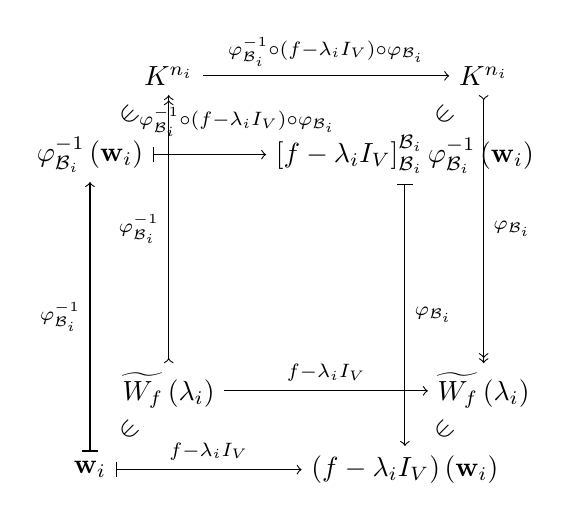
\begin{tikzpicture}[auto]

    \node (a) at (1, 1) {$\widetilde{W_f } \left( \lambda_i \right) $};
    \node (b) at (5, 1) {$\widetilde{W_f } \left( \lambda_i \right) $};
    \node (c) at (1, 5) {$K^{n_i } $};
    \node (d) at (5, 5) {$K^{n_i } $};
    \node (e) at (0, 4) {$\varphi_{{\mathcal B}_i }^{-1} \left( {\bf w}_i \right) $};
    \node (f) at (4, 4) {$\left[ f-\lambda_i I_V \right]_{{\mathcal B}_i }^{{\mathcal B}_i } \varphi_{{\mathcal B}_i }^{-1} \left( {\bf w}_i \right) $};
    \node (g) at (0.5, 4.5) {\rotatebox{45}{$\scriptsize \in $} };
    \node (h) at (4.5, 4.5) {\rotatebox{45}{$\scriptsize \in $} };
    \node (i) at (0, 0) {${\bf w}_i $};
    \node (j) at (4, 0) {$\left( f-\lambda_i I_V \right) \left( {\bf w}_i \right) $};
    \node (k) at (0.5, 0.5) {\rotatebox{45}{$\in $} };
    \node (l) at (4.5, 0.5) {\rotatebox{45}{$\in $} };
    
    \draw [->] (c) to node {$\scriptstyle \varphi_{{\mathcal B}_i }^{-1} \circ \left( f-\lambda_i I_V \right) \circ \varphi_{{\mathcal B}_i } $} (d);
    \draw [|->] (e) to node[xshift=10pt, yshift=3pt] {$\scriptstyle \varphi_{{\mathcal B}_i }^{-1} \circ \left( f-\lambda_i I_V \right) \circ \varphi_{{\mathcal B}_i } $} (f);
    \draw [>->>] (a) to node {$\scriptstyle \varphi_{{\mathcal B}_i }^{-1} $} (c);
    \draw [|->] (i) to node {$\scriptstyle \varphi_{{\mathcal B}_i }^{-1} $} (e);
    \draw [->] (a) to node {$\scriptstyle f-\lambda_i I_V $} (b);
    \draw [|->] (i) to node {$\scriptstyle f-\lambda_i I_V $} (j);
    \draw [>->>] (d) to node {$\scriptstyle \varphi_{{\mathcal B}_i } $} (b);
    \draw [|->] (f) to node {$\scriptstyle \varphi_{{\mathcal B}_i } $} (j);
    
  \end{tikzpicture} 
\end{center}
例えば、$\mathcal{B} =\left\langle \mathcal{B}_{i} \right\rangle_{i \in \varLambda_{s}}$とおくと、その基底$\mathcal{B}$に関する基底変換における線形同型写像$\varphi_{\mathcal{B}}:K^{n} \rightarrow V$を用いれば、$\forall\mathbf{k} \in K^{n}$に対し、それらの広義の固有空間たち$\widetilde{W_{f}}\left( \lambda_{i} \right)$の元$\mathbf{w}_{i}$を用いて$\varphi_{\mathcal{B}}\left( \mathbf{k} \right) = \bigoplus_{i \in \varLambda_{s}} \mathbf{w}_{i}$と一意的に表されることができて次のようになることから、
\begin{center}
  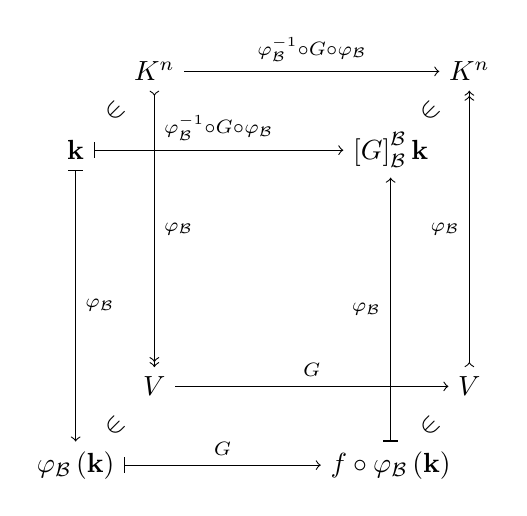
\begin{tikzpicture}[auto]

    \node (a) at (1, 1) {$V$};
    \node (b) at (5, 1) {$V$};
    \node (c) at (1, 5) {$K^n $};
    \node (d) at (5, 5) {$K^n $};
    \node (e) at (0, 4) {${\bf k} $};
    \node (f) at (4, 4) {$\left[ G\right]_{{\mathcal B} }^{{\mathcal B} } {\bf k} $};
    \node (g) at (0.5, 4.5) {\rotatebox{45}{$\scriptsize \in $} };
    \node (h) at (4.5, 4.5) {\rotatebox{45}{$\scriptsize \in $} };
    \node (i) at (0, 0) {$\varphi_{\mathcal B} \left( {\bf k} \right) $};
    \node (j) at (4, 0) {$f\circ \varphi_{\mathcal B} \left( {\bf k} \right) $};
    \node (k) at (0.5, 0.5) {\rotatebox{45}{$\in $} };
    \node (l) at (4.5, 0.5) {\rotatebox{45}{$\in $} };
    
    \draw [->] (c) to node {$\scriptstyle \varphi_{{\mathcal B} }^{-1} \circ G\circ \varphi_{{\mathcal B} } $} (d);
    \draw [|->] (e) to node {$\scriptstyle \varphi_{{\mathcal B} }^{-1} \circ G\circ \varphi_{{\mathcal B} } $} (f);
    \draw [>->>] (c) to node {$\scriptstyle \varphi_{{\mathcal B} } $} (a);
    \draw [|->] (e) to node {$\scriptstyle \varphi_{{\mathcal B} } $} (i);
    \draw [->] (a) to node {$\scriptstyle G $} (b);
    \draw [|->] (i) to node {$\scriptstyle G $} (j);
    \draw [>->>] (b) to node {$\scriptstyle \varphi_{{\mathcal B} } $} (d);
    \draw [|->] (j) to node {$\scriptstyle \varphi_{{\mathcal B} } $} (f);
    
  \end{tikzpicture} 
\end{center}
次のようになる。
\begin{align*}
\varphi_{\mathcal{B}}^{- 1} \circ G \circ \varphi_{\mathcal{B}}\left( \mathbf{k} \right) &= \varphi_{\mathcal{B}}^{- 1} \circ G\left( \bigoplus_{i \in \varLambda_{s}} \mathbf{w}_{i} \right) \\
&= \sum_{i \in \varLambda_{s}} {\varphi_{\mathcal{B}}^{- 1} \circ G\left( \mathbf{w}_{i} \right)} \\
&= \sum_{i \in \varLambda_{s}} {\varphi_{\mathcal{B}}^{- 1} \circ \varphi_{\mathcal{B}_{i}} \circ \varphi_{\mathcal{B}_{i}}^{- 1} \circ G \circ \varphi_{\mathcal{B}_{i}} \circ \varphi_{\mathcal{B}_{i}}^{- 1}\left( \mathbf{w}_{i} \right)} \\
&= \sum_{i \in \varLambda_{s}} {\varphi_{\mathcal{B}}^{- 1} \circ \varphi_{\mathcal{B}_{i}} \circ \varphi_{\mathcal{B}_{i}}^{- 1} \circ \left( f - \lambda_{i}I_{V} \right) \circ \varphi_{\mathcal{B}_{i}} \circ \varphi_{\mathcal{B}_{i}}^{- 1}\left( \mathbf{w}_{i} \right)} \\
&= \sum_{i \in \varLambda_{s}} {\varphi_{\mathcal{B}}^{- 1} \circ \varphi_{\mathcal{B}_{i}}\left( \left[f - \lambda_{i}I_{V} \right]_{\mathcal{B}_{i}}^{\mathcal{B}_{i}}\varphi_{\mathcal{B}_{i}}^{- 1}\left( \mathbf{w}_{i} \right) \right)} \\
&= \begin{pmatrix}
\left[f - \lambda_{1}I_{V} \right]_{\mathcal{B}_{1}}^{\mathcal{B}_{1}}\varphi_{\mathcal{B}_{1}}^{- 1}\left( \mathbf{w}_{1} \right) \\
\mathbf{0} \\
 \vdots \\
\mathbf{0} \\
\end{pmatrix} + \begin{pmatrix}
\mathbf{0} \\
\left[f - \lambda_{2}I_{V} \right]_{\mathcal{B}_{2}}^{\mathcal{B}_{2}}\varphi_{\mathcal{B}_{2}}^{- 1}\left( \mathbf{w}_{2} \right) \\
 \vdots \\
\mathbf{0} \\
\end{pmatrix} + \cdots + \begin{pmatrix}
\mathbf{0} \\
\mathbf{0} \\
 \vdots \\
\left[f - \lambda_{s}I_{V} \right]_{\mathcal{B}_{s}}^{\mathcal{B}_{s}}\varphi_{\mathcal{B}_{s}}^{- 1}\left( \mathbf{w}_{s} \right) \\
\end{pmatrix} \\
&= \begin{pmatrix}
J\left( 0;Q_{1} \right)\varphi_{\mathcal{B}_{1}}^{- 1}\left( \mathbf{w}_{1} \right) \\
\mathbf{0} \\
 \vdots \\
\mathbf{0} \\
\end{pmatrix} + \begin{pmatrix}
\mathbf{0} \\
J\left( 0;Q_{2} \right)\varphi_{\mathcal{B}_{2}}^{- 1}\left( \mathbf{w}_{2} \right) \\
 \vdots \\
\mathbf{0} \\
\end{pmatrix} + \cdots + \begin{pmatrix}
\mathbf{0} \\
\mathbf{0} \\
 \vdots \\
J\left( 0;Q_{s} \right)\varphi_{\mathcal{B}_{s}}^{- 1}\left( \mathbf{w}_{s} \right) \\
\end{pmatrix} \\
&= \begin{pmatrix}
J\left( 0;Q_{1} \right) \\
O \\
 \vdots \\
O \\
\end{pmatrix}\varphi_{\mathcal{B}_{1}}^{- 1}\left( \mathbf{w}_{1} \right) + \begin{pmatrix}
O \\
J\left( 0;Q_{2} \right) \\
 \vdots \\
O \\
\end{pmatrix}\varphi_{\mathcal{B}_{2}}^{- 1}\left( \mathbf{w}_{2} \right) + \cdots + \begin{pmatrix}
O \\
O \\
 \vdots \\
J\left( 0;Q_{s} \right) \\
\end{pmatrix}\varphi_{\mathcal{B}_{s}}^{- 1}\left( \mathbf{w}_{s} \right) \\
&= \begin{pmatrix}
J\left( 0;Q_{1} \right) & \  & \  & O \\
\  & J\left( 0;Q_{2} \right) & \  & \  \\
\  & \  & \ddots & \  \\
O & \  & \  & J\left( 0;Q_{s} \right) \\
\end{pmatrix}\begin{pmatrix}
\varphi_{\mathcal{B}_{1}}^{- 1}\left( \mathbf{w}_{1} \right) \\
\varphi_{\mathcal{B}_{2}}^{- 1}\left( \mathbf{w}_{2} \right) \\
 \vdots \\
\varphi_{\mathcal{B}_{s}}^{- 1}\left( \mathbf{w}_{s} \right) \\
\end{pmatrix}
\end{align*}
ここで、次のようになるので、
\begin{align*}
\begin{pmatrix}
\varphi_{\mathcal{B}_{1}}^{- 1}\left( \mathbf{w}_{1} \right) \\
\varphi_{\mathcal{B}_{2}}^{- 1}\left( \mathbf{w}_{2} \right) \\
 \vdots \\
\varphi_{\mathcal{B}_{s}}^{- 1}\left( \mathbf{w}_{s} \right) \\
\end{pmatrix} &= \begin{pmatrix}
\varphi_{\mathcal{B}_{1}}^{- 1}\left( \mathbf{w}_{1} \right) \\
\mathbf{0} \\
 \vdots \\
\mathbf{0} \\
\end{pmatrix} + \begin{pmatrix}
\mathbf{0} \\
\varphi_{\mathcal{B}_{2}}^{- 1}\left( \mathbf{w}_{2} \right) \\
 \vdots \\
\mathbf{0} \\
\end{pmatrix} + \cdots + \begin{pmatrix}
\mathbf{0} \\
\mathbf{0} \\
 \vdots \\
\varphi_{\mathcal{B}_{s}}^{- 1}\left( \mathbf{w}_{s} \right) \\
\end{pmatrix} \\
&= \varphi_{\mathcal{B}}^{- 1}\left( \mathbf{w}_{1} \right) + \varphi_{\mathcal{B}}^{- 1}\left( \mathbf{w}_{2} \right) + \cdots + \varphi_{\mathcal{B}}^{- 1}\left( \mathbf{w}_{s} \right) \\
&= \varphi_{\mathcal{B}}^{- 1}\left( \bigoplus_{j \in \varLambda_{s}} \mathbf{w}_{j} \right) \\
&= \varphi_{\mathcal{B}}^{- 1} \circ \varphi_{\mathcal{B}}\left( \mathbf{k} \right) = \mathbf{k}
\end{align*}
次のようになる。
\begin{align*}
\varphi_{\mathcal{B}}^{- 1} \circ G \circ \varphi_{\mathcal{B}}\left( \mathbf{k} \right) = \begin{pmatrix}
J\left( 0;Q_{1} \right) & \  & \  & O \\
\  & J\left( 0;Q_{2} \right) & \  & \  \\
\  & \  & \ddots & \  \\
O & \  & \  & J\left( 0;Q_{s} \right) \\
\end{pmatrix}\mathbf{k}
\end{align*}
以上より、次式が成り立つ。
\begin{align*}
[G]_{\mathcal{B}}^{\mathcal{B}} = \begin{pmatrix}
J\left( 0;Q_{1} \right) & \  & \  & O \\
\  & J\left( 0;Q_{2} \right) & \  & \  \\
\  & \  & \ddots & \  \\
O & \  & \  & J\left( 0;Q_{s} \right) \\
\end{pmatrix}
\end{align*}
これにより、次のようになる。
\begin{align*}
[R]_{\mathcal{B}}^{\mathcal{B}} &= [G + R - G]_{\mathcal{B}}^{\mathcal{B}} \\
&= [G + R]_{\mathcal{B}}^{\mathcal{B}} - [G]_{\mathcal{B}}^{\mathcal{B}} \\
&= [f]_{\mathcal{B}}^{\mathcal{B}} - [G]_{\mathcal{B}}^{\mathcal{B}} \\
&= \begin{pmatrix}
J\left( \lambda_{1};Q_{1} \right) & \  & \  & O \\
\  & J\left( \lambda_{2};Q_{2} \right) & \  & \  \\
\  & \  & \ddots & \  \\
O & \  & \  & J\left( \lambda_{s};Q_{s} \right) \\
\end{pmatrix} - \begin{pmatrix}
J\left( 0;Q_{1} \right) & \  & \  & O \\
\  & J\left( 0;Q_{2} \right) & \  & \  \\
\  & \  & \ddots & \  \\
O & \  & \  & J\left( 0;Q_{s} \right) \\
\end{pmatrix} \\
&= \begin{pmatrix}
\lambda_{1}I_{n_{1}} & \  & \  & O \\
\  & \lambda_{2}I_{n_{2}} & \  & \  \\
\  & \  & \ddots & \  \\
O & \  & \  & \lambda_{s}I_{n_{s}} \\
\end{pmatrix}
\end{align*}
したがって、その線形写像$R$は対角化可能である。\par
よって、対角化可能な線形写像$R:V \rightarrow V$と冪零変換$G:V \rightarrow V$が存在して$f = R + G$が成り立つかつ、$R \circ G = G \circ R$が成り立つ。\par
より詳しくいえば、分解定理より$V = \bigoplus_{i \in \varLambda_{s}} {\widetilde{W_{f}}\left( \lambda_{i} \right)}$が成り立つので、そのvector空間$V$からその広義の固有空間$\widetilde{W_{f}}\left( \lambda_{i} \right)$への直和分解から定まる射影$P_{i}$を用いて$\forall\mathbf{v} \in V$に対し、それらの広義の固有空間たち$\widetilde{W_{f}}\left( \lambda_{i} \right)$の元$\mathbf{w}_{i}$を用いて$\mathbf{v} = \bigoplus_{i \in \varLambda_{s}} \mathbf{w}_{i}$と一意的に表されることができて次のようになる。
\begin{align*}
R\left( \mathbf{v} \right) &= R\left( \bigoplus_{i \in \varLambda_{s}} \mathbf{w}_{i} \right) \\
&= \sum_{i \in \varLambda_{s}} {R\left( \mathbf{w}_{i} \right)} \\
&= \sum_{i \in \varLambda_{s}} {\lambda_{i}I_{V}\left( \mathbf{w}_{i} \right)} \\
&= \sum_{i \in \varLambda_{s}} {\lambda_{i}\mathbf{w}_{i}} \\
&= \sum_{i \in \varLambda_{s}} {\lambda_{i}P_{i}\left( \bigoplus_{j \in \varLambda_{s}} \mathbf{w}_{j} \right)} \\
&= \sum_{i \in \varLambda_{s}} {\lambda_{i}P_{i}\left( \mathbf{v} \right)} \\
&= \left( \sum_{i \in \varLambda_{s}} {\lambda_{i}P_{i}} \right)\left( \mathbf{v} \right)
\end{align*}
したがって、$R = \sum_{i \in \varLambda_{s}} {\lambda_{i}P_{i}}$が成り立つ。
\end{proof}
%\hypertarget{ux540cux6642ux5bfeux89d2ux5316}{%
\subsubsection{同時対角化}%\label{ux540cux6642ux5bfeux89d2ux5316}}
\begin{thm}\label{2.2.7.2}
代数的閉体$K$上の$n$次元vector空間$V$における対角化可能な線形写像$R:V \rightarrow V$、$R$-不変なそのvector空間$V$の部分空間$W$が与えられたとき、線形写像$R|W:W \rightarrow W$も対角化可能である。
\end{thm}
\begin{proof}
代数的閉体$K$上の$n$次元vector空間$V$における対角化可能な線形写像$R:V \rightarrow V$、$R$-不変なそのvector空間$V$の部分空間$W$が与えられたとき、定理\ref{2.2.6.12}よりその線形写像$R$の最小多項式$\varphi_{R}$がその線形写像$R$の$i \in \varLambda_{s}$なる互いに異なる固有値たち$\lambda_{i}$を用いて次式を満たすかつ、
\begin{align*}
\varphi_{R} = \prod_{i \in \varLambda_{s}} \left( X - \lambda_{i} \right)
\end{align*}
Hamilton-Cayleyの定理より$\varphi_{R}(R) = 0$が成り立つので、もちろん、$\varphi_{R}\left( R|W \right) = 0$が成り立つ。したがって、その線形写像$R$の最小多項式$\varphi_{R}$、その線形写像$R|W$の最小多項式$\varphi_{R|W}$において、定理\ref{2.2.6.7}よりその多項式$\varphi_{R}$はその多項式$\varphi_{R|W}$で割り切れる。ゆえに、その集合$\varLambda_{s}$の部分集合$\varLambda'$を用いて次式が成り立つ。
\begin{align*}
\varphi_{R|W} = \prod_{i \in \varLambda'} \left( X - \lambda_{i} \right)
\end{align*}
これにより、定理\ref{2.2.6.12}よりその線形写像$R|W$もその部分空間$W$で対角化可能である。
\end{proof}
\begin{thm}[同時対角化]\label{2.2.7.3}
代数的閉体$K$上の$n$次元vector空間$V$における対角化可能な線形写像たち$R:V \rightarrow V$、$S:V \rightarrow V$が与えられたとき、$S \circ R = R \circ S$が成り立つなら、そのvector空間$V$のある基底$\mathcal{B}$が存在してこれに関するそれらの線形写像たち$R$、$S$の表現行列たち$[R]_{\mathcal{B}}^{\mathcal{B}}$、$[S]_{\mathcal{B}}^{\mathcal{B}}$が対角行列となる。\par
この定理での基底$\mathcal{B}$をとること、あるいは、この定理を同時対角化という。このことから明らかに、$\forall k,l \in K$に対し、線形写像$kR + lS$もその基底$\mathcal{B}$で対角化可能である。
\end{thm}
\begin{proof}
代数的閉体$K$上の$n$次元vector空間$V$における対角化可能な線形写像たち$R:V \rightarrow V$、$S:V \rightarrow V$が与えられたとき、$S \circ R = R \circ S$が成り立つなら、その線形写像$R$の互いに異なる$i \in \varLambda_{s}$なる固有値たち$\lambda_{i}$を用いれば、その線形写像$R$は対角化可能であるから、その固有値$\lambda_{i}$に対する固有空間$W_{R}\left( \lambda_{i} \right)$を用いれば、定理\ref{2.2.4.15}より$V = \bigoplus_{i \in \varLambda_{s}} {W_{R}\left( \lambda_{i} \right)}$が成り立つ。ここで、$\forall i \in \varLambda_{s}$に対し、その固有空間$W_{R}\left( \lambda_{i} \right)$は定理\ref{2.2.5.9}より$R$-不変で、$\forall\mathbf{w} \in W_{R}\left( \lambda_{i} \right)$に対し、次のようになることから、
\begin{align*}
R\left( S\left( \mathbf{w} \right) \right) &= R \circ S\left( \mathbf{w} \right) \\
&= S \circ R\left( \mathbf{w} \right) \\
&= S\left( R\left( \mathbf{w} \right) \right) \\
&= S\left( \lambda_{i}\mathbf{w} \right) = \lambda_{i}S\left( \mathbf{w} \right)
\end{align*}
$S\left( \mathbf{w} \right) \in W_{R}\left( \lambda_{i} \right)$が成り立つので、その固有空間$W_{R}\left( \lambda_{i} \right)$は$S$-不変でもある。ここで、その線形写像$S$は対角化可能なので、定理\ref{2.2.7.2}より線形写像$S|W_{R}\left( \lambda_{i} \right)$も対角化可能である。したがって、あるその固有空間$W_{R}\left( \lambda_{i} \right)$の基底$\mathcal{B}_{i}$が存在して、これに関するその線形写像$S|W_{R}\left( \lambda_{i} \right)$の表現行列$\left[S|W_{R}\left( \lambda_{i} \right) \right]_{\mathcal{B}_{i}}^{\mathcal{B}_{i}}$は対角行列である。ここで、$\mathcal{B} =\left\langle \mathcal{B}_{i} \right\rangle_{i \in \varLambda_{s}}$とおかれれば、その基底$\mathcal{B}$に関する基底変換における線形同型写像$\varphi_{\mathcal{B}}:K^{n} \rightarrow V$を用いれば、次のようになることから、
\begin{center}
  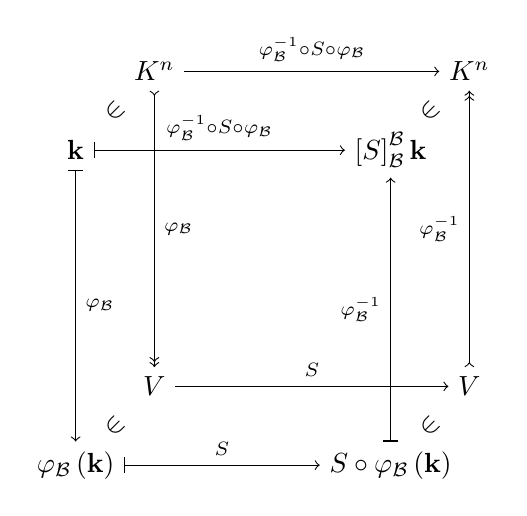
\begin{tikzpicture}[auto]

    \node (a) at (1, 1) {$V$};
    \node (b) at (5, 1) {$V$};
    \node (c) at (1, 5) {$K^n $};
    \node (d) at (5, 5) {$K^n $};
    \node (e) at (0, 4) {${\bf k} $};
    \node (f) at (4, 4) {$\left[ S\right]_{{\mathcal B} }^{{\mathcal B} } {\bf k} $};
    \node (g) at (0.5, 4.5) {\rotatebox{45}{$\scriptsize \in $} };
    \node (h) at (4.5, 4.5) {\rotatebox{45}{$\scriptsize \in $} };
    \node (i) at (0, 0) {$\varphi_{\mathcal B} \left( {\bf k} \right) $};
    \node (j) at (4, 0) {$S\circ \varphi_{\mathcal B} \left( {\bf k} \right) $};
    \node (k) at (0.5, 0.5) {\rotatebox{45}{$\in $} };
    \node (l) at (4.5, 0.5) {\rotatebox{45}{$\in $} };
    
    \draw [->] (c) to node {$\scriptstyle \varphi_{{\mathcal B} }^{-1} \circ S \circ \varphi_{{\mathcal B} } $} (d);
    \draw [|->] (e) to node {$\scriptstyle \varphi_{{\mathcal B} }^{-1} \circ S \circ \varphi_{{\mathcal B} } $} (f);
    \draw [>->>] (c) to node {$\scriptstyle \varphi_{{\mathcal B} } $} (a);
    \draw [|->] (e) to node {$\scriptstyle \varphi_{{\mathcal B} } $} (i);
    \draw [->] (a) to node {$\scriptstyle S$} (b);
    \draw [|->] (i) to node {$\scriptstyle S$} (j);
    \draw [>->>] (b) to node {$\scriptstyle \varphi_{{\mathcal B} }^{-1} $} (d);
    \draw [|->] (j) to node {$\scriptstyle \varphi_{{\mathcal B} }^{-1} $} (f);
    
  \end{tikzpicture} 
\end{center}
$\forall\mathbf{k} \in K^{n}$に対し、その固有空間$W_{R}\left( \lambda_{i} \right)$の元$\mathbf{w}_{i}$を用いて$\mathbf{v} = \bigoplus_{i \in \varLambda_{s}} \mathbf{w}_{i}$と一意的に表されることができるので、$S|W_{R}\left( \lambda_{i} \right) = \left( W_{R}\left( \lambda_{i} \right) \rightarrow W_{R}\left( \lambda_{i} \right);\mathbf{v} \mapsto S\left( \mathbf{v} \right) \right)$と同一視すると次のようになる。
\begin{align*}
\varphi_{\mathcal{B}}^{- 1} \circ S \circ \varphi_{\mathcal{B}}\left( \mathbf{k} \right) &= \varphi_{\mathcal{B}}^{- 1} \circ S\left( \bigoplus_{i \in \varLambda_{s}} \mathbf{w}_{i} \right) \\
&= \sum_{i \in \varLambda_{s}} {\varphi_{\mathcal{B}}^{- 1} \circ S\left( \mathbf{w}_{i} \right)} \\
&= \sum_{i \in \varLambda_{s}} {\varphi_{\mathcal{B}}^{- 1} \circ \varphi_{\mathcal{B}_{i}} \circ \varphi_{\mathcal{B}_{i}}^{- 1} \circ S|W_{R}\left( \lambda_{i} \right) \circ \varphi_{\mathcal{B}_{i}} \circ \varphi_{\mathcal{B}_{i}}^{- 1}\left( \mathbf{w}_{i} \right)} \\
&= \sum_{i \in \varLambda_{s}} {\varphi_{\mathcal{B}}^{- 1} \circ \varphi_{\mathcal{B}_{i}}\left( \left[S|W_{R}\left( \lambda_{i} \right) \right]_{\mathcal{B}_{i}}^{\mathcal{B}_{i}}\varphi_{\mathcal{B}_{i}}^{- 1}\left( \mathbf{w}_{i} \right) \right)} \\
&= \begin{pmatrix}
\left[S|W_{R}\left( \lambda_{1} \right) \right]_{\mathcal{B}_{1}}^{\mathcal{B}_{1}}\varphi_{\mathcal{B}_{1}}^{- 1}\left( \mathbf{w}_{1} \right) \\
\mathbf{0} \\
 \vdots \\
\mathbf{0} \\
\end{pmatrix} + \begin{pmatrix}
\mathbf{0} \\
\left[S|W_{R}\left( \lambda_{2} \right) \right]_{\mathcal{B}_{2}}^{\mathcal{B}_{2}}\varphi_{\mathcal{B}_{2}}^{- 1}\left( \mathbf{w}_{2} \right) \\
 \vdots \\
\mathbf{0} \\
\end{pmatrix} + \cdots + \begin{pmatrix}
\mathbf{0} \\
\mathbf{0} \\
 \vdots \\
\left[S|W_{R}\left( \lambda_{s} \right) \right]_{\mathcal{B}_{s}}^{\mathcal{B}_{s}}\varphi_{\mathcal{B}_{s}}^{- 1}\left( \mathbf{w}_{s} \right) \\
\end{pmatrix} \\
&= \begin{pmatrix}
\left[S|W_{R}\left( \lambda_{1} \right) \right]_{\mathcal{B}_{1}}^{\mathcal{B}_{1}} & \  & \  & O \\
\  & \left[S|W_{R}\left( \lambda_{2} \right) \right]_{\mathcal{B}_{2}}^{\mathcal{B}_{2}} & \  & \  \\
\  & \  & \ddots & \  \\
O & \  & \  & \left[S|W_{R}\left( \lambda_{s} \right) \right]_{\mathcal{B}_{s}}^{\mathcal{B}_{s}} \\
\end{pmatrix}\begin{pmatrix}
\varphi_{\mathcal{B}_{1}}^{- 1}\left( \mathbf{w}_{1} \right) \\
\varphi_{\mathcal{B}_{2}}^{- 1}\left( \mathbf{w}_{2} \right) \\
 \vdots \\
\varphi_{\mathcal{B}_{s}}^{- 1}\left( \mathbf{w}_{s} \right) \\
\end{pmatrix}
\end{align*}
ここで、次のようになるので、
\begin{align*}
\begin{pmatrix}
\varphi_{\mathcal{B}_{1}}^{- 1}\left( \mathbf{w}_{1} \right) \\
\varphi_{\mathcal{B}_{2}}^{- 1}\left( \mathbf{w}_{2} \right) \\
 \vdots \\
\varphi_{\mathcal{B}_{s}}^{- 1}\left( \mathbf{w}_{s} \right) \\
\end{pmatrix} &= \begin{pmatrix}
\varphi_{\mathcal{B}_{1}}^{- 1}\left( \mathbf{w}_{1} \right) \\
\mathbf{0} \\
 \vdots \\
\mathbf{0} \\
\end{pmatrix} + \begin{pmatrix}
\mathbf{0} \\
\varphi_{\mathcal{B}_{2}}^{- 1}\left( \mathbf{w}_{2} \right) \\
 \vdots \\
\mathbf{0} \\
\end{pmatrix} + \cdots + \begin{pmatrix}
\mathbf{0} \\
\mathbf{0} \\
 \vdots \\
\varphi_{\mathcal{B}_{s}}^{- 1}\left( \mathbf{w}_{s} \right) \\
\end{pmatrix} \\
&= \varphi_{\mathcal{B}}^{- 1}\left( \mathbf{w}_{1} \right) + \varphi_{\mathcal{B}}^{- 1}\left( \mathbf{w}_{2} \right) + \cdots + \varphi_{\mathcal{B}}^{- 1}\left( \mathbf{w}_{s} \right) \\
&= \varphi_{\mathcal{B}}^{- 1}\left( \bigoplus_{j \in \varLambda_{s}} \mathbf{w}_{j} \right) \\
&= \varphi_{\mathcal{B}}^{- 1} \circ \varphi_{\mathcal{B}}\left( \mathbf{k} \right) = \mathbf{k}
\end{align*}
次のようになる。
\begin{align*}
\varphi_{\mathcal{B}}^{- 1} \circ S \circ \varphi_{\mathcal{B}}\left( \mathbf{k} \right) = \begin{pmatrix}
\left[S|W_{R}\left( \lambda_{1} \right) \right]_{\mathcal{B}_{1}}^{\mathcal{B}_{1}} & \  & \  & O \\
\  & \left[S|W_{R}\left( \lambda_{2} \right) \right]_{\mathcal{B}_{2}}^{\mathcal{B}_{2}} & \  & \  \\
\  & \  & \ddots & \  \\
O & \  & \  & \left[S|W_{R}\left( \lambda_{s} \right) \right]_{\mathcal{B}_{s}}^{\mathcal{B}_{s}} \\
\end{pmatrix}\mathbf{k}
\end{align*}
したがって、次式が成り立つので、
\begin{align*}
[S]_{\mathcal{B}}^{\mathcal{B}} = \begin{pmatrix}
\left[S|W_{R}\left( \lambda_{1} \right) \right]_{\mathcal{B}_{1}}^{\mathcal{B}_{1}} & \  & \  & O \\
\  & \left[S|W_{R}\left( \lambda_{2} \right) \right]_{\mathcal{B}_{2}}^{\mathcal{B}_{2}} & \  & \  \\
\  & \  & \ddots & \  \\
O & \  & \  & \left[S|W_{R}\left( \lambda_{s} \right) \right]_{\mathcal{B}_{s}}^{\mathcal{B}_{s}} \\
\end{pmatrix}
\end{align*}
その線形写像$S$のその基底$\mathcal{B}$に関する表現行列$[S]_{\mathcal{B}}^{\mathcal{B}}$は対角行列となり、このとき、その基底$\mathcal{B}$をなすvectorsはいづれもその線形写像$R$の固有vectorであるから、定理\ref{2.2.2.14}よりその線形写像$R$のその基底$\mathcal{B}$に関する表現行列$[R]_{\mathcal{B}}^{\mathcal{B}}$も対角行列となる。よって、そのvector空間$V$のある基底$\mathcal{B}$が存在してこれに関するそれらの線形写像たち$R$、$S$の表現行列たち$[R]_{\mathcal{B}}^{\mathcal{B}}$、$[S]_{\mathcal{B}}^{\mathcal{B}}$が対角行列となる。\par
これにより、$\forall k,l \in K$に対し、$[kR + lS]_{\mathcal{B}}^{\mathcal{B}} = k[R]_{\mathcal{B}}^{\mathcal{B}} + l[S]_{\mathcal{B}}^{\mathcal{B}}$が成り立つことから、行列$[kR + lS]_{\mathcal{B}}^{\mathcal{B}}$も対角行列となり、したがって、線形写像$kR + lS$もその基底$\mathcal{B}$で対角化可能である。
\end{proof}
\begin{thm}\label{2.2.7.4}
代数的閉体$K$上の$n$次元vector空間$V$における冪零変換たち$G:V \rightarrow V$、$H:V \rightarrow V$が与えられたとき、$H \circ G = G \circ H$が成り立つなら、$\forall k,l \in K$に対し、線形写像$kG + lH$も冪零変換である。
\end{thm}
\begin{proof}
代数的閉体$K$上の$n$次元vector空間$V$における指数それぞれ$p$、$q$の冪零変換たち$G:V \rightarrow V$、$H:V \rightarrow V$が与えられたとき、$H \circ G = G \circ H$が成り立つなら、$\forall k,l \in K$に対し、定理\ref{2.1.2.10}と二項定理より$j = p + q - 1$とおいて次のようになる。
\begin{align*}
(kG + lH)^{j} &= \sum_{i \in \varLambda_{j} \cup \left\{ 0 \right\}} {\frac{j!}{i!(j - i)!}(kG)^{i} \circ (lH)^{j - i}} \\
&= \sum_{\scriptsize \begin{matrix} i \in \varLambda_{j} \cup \left\{ 0 \right\} \\p \leq i \\\end{matrix}} {\frac{j!}{i!(j - i)!}(kG)^{i} \circ (lH)^{j - i}} + \sum_{\scriptsize \begin{matrix} i \in \varLambda_{j} \cup \left\{ 0 \right\} \\i < p \\\end{matrix}} {\frac{j!}{i!(j - i)!}(kG)^{i} \circ (lH)^{j - i}} \\
&= \sum_{\scriptsize \begin{matrix} i \in \varLambda_{j} \cup \left\{ 0 \right\} \\p \leq i \\\end{matrix}} {\frac{j!}{i!(j - i)!}(kG)^{i} \circ (lH)^{j - i}} + \sum_{\scriptsize \begin{matrix} i \in \varLambda_{j} \cup \left\{ 0 \right\} \\q \leq j - i \\\end{matrix}} {\frac{j!}{i!(j - i)!}(kG)^{i} \circ (lH)^{j - i}} \\
&= \sum_{\scriptsize \begin{matrix} i \in \varLambda_{j} \cup \left\{ 0 \right\} \\p \leq i \\\end{matrix}} {\frac{j!}{i!(j - i)!}k^{i}l^{j - i}H^{j - i} \circ G^{i}} + \sum_{\scriptsize \begin{matrix} i \in \varLambda_{j} \cup \left\{ 0 \right\} \\q \leq j - i \\\end{matrix}} {\frac{j!}{i!(j - i)!}k^{i}l^{j - i}G^{i} \circ H^{j - i}} \\
&= \sum_{\scriptsize \begin{matrix} i \in \varLambda_{j} \cup \left\{ 0 \right\} \\p \leq i \\\end{matrix}} {\frac{j!}{i!(j - i)!}k^{i}l^{j - i}H^{j - i} \circ G^{i - p} \circ G^{p}} \\
&\quad + \sum_{\scriptsize \begin{matrix}  \in \varLambda_{j} \cup \left\{ 0 \right\} \\q \leq j - i \\\end{matrix}} {\frac{j!}{i!(j - i)!}k^{i}l^{j - i}G^{i} \circ H^{j - i - q} \circ H^{q}} \\
&= \sum_{\scriptsize \begin{matrix} i \in \varLambda_{j} \cup \left\{ 0 \right\} \\p \leq i \\\end{matrix}} {\frac{j!}{i!(j - i)!}k^{i}l^{j - i}H^{j - i} \circ G^{i - p} \circ 0} \\
&\quad + \sum_{\scriptsize \begin{matrix} i \in \varLambda_{j} \cup \left\{ 0 \right\} \\q \leq j - i \\\end{matrix}} {\frac{j!}{i!(j - i)!}k^{i}l^{j - i}G^{i} \circ H^{j - i - q} \circ 0} \\
&= \sum_{\scriptsize \begin{matrix} i \in \varLambda_{j} \cup \left\{ 0 \right\} \\ p \leq i \\\end{matrix}} 0 + \sum_{i \in \varLambda_{j} \cup \left\{ 0 \right\} ,q \leq j - i } 0 = 0
\end{align*}
よって、その線形写像$kG + lH$も冪零変換である。
\end{proof}
%\hypertarget{jordanux5206ux89e3ux306eux4e00ux610fux6027}{%
\subsubsection{Jordan分解の一意性}%\label{jordanux5206ux89e3ux306eux4e00ux610fux6027}}
\begin{thm}\label{2.2.7.5}
代数的閉体$K$上の$n$次元vector空間$V$における線形写像$T:V \rightarrow V$が対角化可能であるかつ、冪零変換であるなら、$T = 0$が成り立つ。
\end{thm}
\begin{proof}
代数的閉体$K$上の$n$次元vector空間$V$における線形写像$T:V \rightarrow V$が対角化可能であるかつ、冪零変換であるなら、その線形写像$T$の固有値たち$\lambda_{i}$を用いてある基底$\mathcal{B}$が存在してこれに関するその線形写像$T$の表現行列$[T]_{\mathcal{B}}^{\mathcal{B}}$が次式のように表される。
\begin{align*}
[T]_{\mathcal{B}}^{\mathcal{B}} = \begin{pmatrix}
\lambda_{1} & \  & \  & O \\
\  & \lambda_{2} & \  & \  \\
\  & \  & \ddots & \  \\
O & \  & \  & \lambda_{n} \\
\end{pmatrix}
\end{align*}
ここで、定理\ref{2.2.2.6}、定理\ref{2.2.5.1}より$\forall i \in \varLambda_{n}$に対し、$\lambda_{i} = 0$が成り立つことになる。したがって、$[T]_{\mathcal{B}}^{\mathcal{B}} = 0$が成り立つので、$T = 0$が成り立つ。
\end{proof}
\begin{thm}[Jordan分解の一意性]\label{2.2.7.6}
代数的閉体$K$上の$n$次元vector空間$V$における任意の線形写像$f:V \rightarrow V$が$S + N$分解により対角化可能な線形写像$R:V \rightarrow V$と冪零変換$G:V \rightarrow V$を用いて$G \circ R = R \circ G$が成り立つかつ、$f = R + G$と表されることができるとき、このような線形写像たち$R$、$G$はただ1つ存在する。この定理をJoedan分解の一意性という。
\end{thm}
\begin{proof}
代数的閉体$K$上の$n$次元vector空間$V$における任意の線形写像$f:V \rightarrow V$がJordan分解により対角化可能な線形写像たち$R:V \rightarrow V$、$S:V \rightarrow V$と冪零変換たち$G:V \rightarrow V$、$H:V \rightarrow V$を用いて$G \circ R = R \circ G$、$H \circ S = S \circ H$が成り立つかつ、$f = R + G = S + H$と表されることができるとする。さらに、その線形写像$f$の互いに異なる固有値の族$\left\{ \lambda_{i} \right\}_{i \in \varLambda_{s}}$が与えられたとする。\par
その線形写像$f$の固有多項式$\varPhi_{f}$の変数$X$にその線形写像$f$を代入した写像$\varPhi_{f}(f)$がHamilton-Cayleyの定理より$\varPhi_{f}(f) = 0$を満たすかつ、その多項式環$K[X]$が単項ideal整域をなすことと素元分解の基本定理よりその固有多項式$\varPhi_{f}$はその多項式環$K[X]$の多項式であるので、$\varPhi_{f} = \prod_{i \in \varLambda_{s}} \left( X - \overline{\lambda_{i}} \right)^{n_{i}}$と表されることができる。$\pi_{i} = \left( X - \overline{\lambda_{i}} \right)^{n_{i}}$とおくと、これらの多項式たち$\pi_{i}$から定まる多項式写像$\pi_{i}$を用いれば、その族$\left\{ \prod_{i' \in \varLambda_{s} \setminus \left\{ i \right\}} {\pi_{i'}} \right\}_{i \in \varLambda_{s}}$の最大公約元は単位元と同伴であることになるので、したがって、次式が成り立つ。
\begin{align*}
K[X] = \sum_{i \in \varLambda_{s}} {K[X]\prod_{i' \in \varLambda_{s} \setminus \left\{ i \right\}} {\pi_{i'}}}
\end{align*}
これにより、その多項式環$K[X]$の族$\left\{ \kappa_{i} \right\}_{i \in \varLambda_{s}}$が存在して次式が成り立つ。
\begin{align*}
\overline{1} = \sum_{i \in \varLambda_{s}} {\kappa_{i}\prod_{i' \in \varLambda_{s} \setminus \left\{ i \right\}} {\pi_{i'}}}
\end{align*}
ここで、それらの多項式たち$\kappa_{i}$から定まる多項式写像たちが$\kappa_{i}:K \rightarrow K$とおかれると、恒等写像$I_{V}:V \rightarrow V$を用いて$I_{K} = \sum_{i \in \varLambda_{s}} {\kappa_{i}\prod_{i' \in \varLambda_{s} \setminus \left\{ i \right\}} \pi_{i'}}$が成り立つことになる。ここで、$\kappa_{i}\prod_{i' \in \varLambda_{s} \setminus \left\{ i \right\}} {\pi_{i'}} = p_{i}$とおかれると、$\overline{1} = \sum_{i \in \varLambda_{s}} {p_{i}}$が成り立つかつ、$\forall i,j \in \varLambda_{s}$に対し、$i \neq j$のとき、次のようになる。
\begin{align*}
p_{j}(f) \circ p_{i}(f) &= \kappa_{j}(f) \circ \prod_{i' \in \varLambda_{s} \setminus \left\{ j \right\}} {\pi_{i'}(f)} \circ \kappa_{i}(f) \circ \prod_{i' \in \varLambda_{s} \setminus \left\{ i \right\}} {\pi_{i'}(f)} \\
&= \kappa_{j}(f) \circ \prod_{i' \in \varLambda_{s} \setminus \left\{ i,j \right\}} {\pi_{i'}(f)} \circ \kappa_{i}(f) \circ \left( \prod_{i \in \varLambda_{s}} \pi_{i} \right)(f)
\end{align*}
ここで、$\varPhi_{f} = \prod_{i \in \varLambda_{s}} {\pi_{i}}$が成り立つので、次のようになる。
\begin{align*}
p_{j}(f) \circ p_{i}(f) &= \kappa_{j}(f) \circ \prod_{i' \in \varLambda_{s} \setminus \left\{ i,j \right\}} {\pi_{i'}(f)} \circ \kappa_{i}(f) \circ \varPhi_{f}(f) \\
&= \kappa_{j}(f) \circ \prod_{i' \in \varLambda_{s} \setminus \left\{ i,j \right\}} {\pi_{i'}(f)} \circ \kappa_{i}(f) \circ 0 = 0
\end{align*}
以上より、$P_{i} = p_{i}(f)$とおいて線形写像$P_{i}:V \rightarrow V$の族$\left\{ P_{i} \right\}_{i \in \varLambda_{s}}$が与えられたとき、次のことを満たし、
\begin{itemize}
\item
  $\forall i,j \in \varLambda_{s}$に対し、$i \neq j$が成り立つなら、$P_{j} \circ P_{i} = 0$が成り立つ。
\item
  $i \in \varLambda_{s}$なるそれらの線形写像たち$P_{i}$について、そのvector空間$V$の恒等写像$I_{V}$を用いて$\sum_{i \in \varLambda_{s}} P_{i} = I_{V}$が成り立つ。
\end{itemize}
定理\ref{2.2.1.10}よりしたがって、その線形写像$P_{i}$がそのvector空間$V$からその部分空間$V\left( P_{i} \right)$への射影で次式が成り立つ。
\begin{align*}
V = \bigoplus_{i \in \varLambda_{n}} {V\left( P_{i} \right)}
\end{align*}\par
このとき、$\forall i \in \varLambda_{s}$に対し、次式が成り立つことから、
\begin{align*}
\kappa_{i}\varPhi_{f} &= \kappa_{i}\prod_{i' \in \varLambda_{s}} {\pi_{i'}} \\
&= \kappa_{i}\prod_{i' \in \varLambda_{s} \setminus \left\{ i \right\}} {\pi_{i'}}\pi_{i} \\
&= p_{i}\pi_{i} \\
&= \pi_{i}p_{i}
\end{align*}
次のようになる。
\begin{align*}
\pi_{i}(f) \circ P_{i} = \pi_{i}(f) \circ p_{i}(f) = \kappa_{i}(f) \circ \varPhi_{f}(f) = 0
\end{align*}
これにより、$\forall\mathbf{v} \in V$に対し、$\mathbf{v} \in V\left( P_{i} \right)$が成り立つなら、$\exists\mathbf{w} \in V$に対し、$\mathbf{v} = P_{i}\left( \mathbf{w} \right)$が成り立つので、$\pi_{i}\left( \mathbf{v} \right) = \pi_{i}(f) \circ P_{i}\left( \mathbf{w} \right) = \mathbf{0}$より次のようになる。
\begin{align*}
\mathbf{v} \in \ker{\pi_{i}(f)} = \ker\left( f - \lambda_{i}I_{V} \right)^{n_{i}} = \ker\left( \lambda_{i}I_{V} - f \right)^{n_{i}}
\end{align*}
したがって、$V\left( P_{i} \right) \subseteq \ker\left( \lambda_{i}I_{V} - f \right)^{n_{i}}$が成り立つ。逆に、$\forall\mathbf{v} \in V$に対し、$\mathbf{v} \in \ker\left( \lambda_{i}I_{V} - f \right)^{n_{i}}$が成り立つなら、$\pi_{i}(f)\left( \mathbf{v} \right) = \mathbf{0}$が成り立つかつ、$\forall j \in \varLambda_{s}$に対し、$i \neq j$が成り立つなら、次のようになり、
\begin{align*}
P_{j}\left( \mathbf{v} \right) &= \kappa_{j}(f) \circ \prod_{i' \in \varLambda_{s} \setminus \left\{ j \right\}} {\pi_{i'}(f)}\left( \mathbf{v} \right) \\
&= \kappa_{j}(f) \circ \prod_{i' \in \varLambda_{s} \setminus \left\{ i,j \right\}} {\pi_{i'}(f)} \circ \pi_{i}(f)\left( \mathbf{v} \right) \\
&= \kappa_{j}(f) \circ \prod_{i' \in \varLambda_{s} \setminus \left\{ i,j \right\}} {\pi_{i'}(f)}\left( \pi_{i}(f)\left( \mathbf{v} \right) \right) \\
&= \kappa_{j}(f) \circ \prod_{i' \in \varLambda_{s} \setminus \left\{ i,j \right\}} {\pi_{i'}(f)}\left( \mathbf{0} \right) = \mathbf{0}
\end{align*}
したがって、次のようになる。
\begin{align*}
\mathbf{v} &= \left( \sum_{i' \in \varLambda_{s}} P_{i'} \right)\left( \mathbf{v} \right) \\
&= \sum_{i' \in \varLambda_{s}} {P_{i'}\left( \mathbf{v} \right)} \\
&= \sum_{i' \in \varLambda_{s} \setminus \left\{ i \right\}} {P_{i'}\left( \mathbf{v} \right)} + P_{i}\left( \mathbf{v} \right) \\
&= \sum_{i' \in \varLambda_{s} \setminus \left\{ i \right\}} \mathbf{0} + P_{i}\left( \mathbf{v} \right) = P_{i}\left( \mathbf{v} \right) \in V\left( P_{i} \right)
\end{align*}
これにより、$\ker\left( \lambda_{i}I_{V} - f \right)^{n_{i}} \subseteq V\left( P_{i} \right)$が成り立つ。以上より、$V\left( P_{i} \right) = \ker\left( \lambda_{i}I_{V} - f \right)^{n_{i}}$が成り立つので、次式が成り立つ。
\begin{align*}
V = \bigoplus_{i \in \varLambda_{n}} {\ker\left( \lambda_{i}I_{V} - f \right)^{n_{i}}}
\end{align*}\par
ここで、分解定理より、これらの広義の固有空間たち$\widetilde{W_{f}}\left( \lambda_{i} \right)$を用いて$V = \bigoplus_{i \in \varLambda_{s}} {\widetilde{W_{f}}\left( \lambda_{i} \right)}$が成り立ち、その線形写像$P_{i}$はそのvector空間$V$からその広義の固有空間$\widetilde{W_{f}}\left( \lambda_{i} \right)$への直和分解から定まる射影でもある。このとき、定理\ref{2.2.7.1}より$S = \sum_{i \in \varLambda_{s}} {\lambda_{i}P_{i}}$とおかれるとすると、次のようになることから、
\begin{align*}
\sum_{i \in \varLambda_{s}} {\overline{\lambda_{i}}p_{i}} &= \sum_{i \in \varLambda_{s}} {\overline{\lambda_{i}}\kappa_{i}\prod_{i' \in \varLambda_{s} \setminus \left\{ i \right\}} {\pi_{i'}}} \\
&= \sum_{i \in \varLambda_{s}} {\overline{\lambda_{i}}\kappa_{i}\prod_{i' \in \varLambda_{s} \setminus \left\{ i \right\}} \left( X - \overline{\lambda_{i'}} \right)^{n_{i'}}}
\end{align*}
次のようになるので、
\begin{align*}
S &= \sum_{i \in \varLambda_{s}} {\lambda_{i}P_{i}} \\
&= \sum_{i \in \varLambda_{s}} {\lambda_{i}p_{i}(f)} \\
&= \sum_{i \in \varLambda_{s}} {\lambda_{i}\kappa_{i}(f)\prod_{i' \in \varLambda_{s} \setminus \left\{ i \right\}} \left( f - \lambda_{i'}I_{V} \right)^{n_{i'}}}
\end{align*}
その線形写像$S$は多項式環$K[X]$の多項式$\sum_{i \in \varLambda_{s}} {\overline{\lambda_{i}}\kappa_{i}\prod_{i' \in \varLambda_{s} \setminus \left\{ i \right\}} \left( X - \overline{\lambda_{i'}} \right)^{n_{i'}}}$から定義される多項式写像のその線形写像$f$による像でもあり、したがって、$\sigma = \sum_{j \in \varLambda_{\nu_{i}} \cup \left\{ 0 \right\}} {\overline{p_{ij}}X^{j}}$、$\nu_{i} = \deg{\sum_{i \in \varLambda_{s}} {\overline{\lambda_{i}}\kappa_{i}\prod_{i' \in \varLambda_{s} \setminus \left\{ i \right\}} \left( X - \overline{\lambda_{i'}} \right)^{n_{i'}}}}$とおかれると、次のようになるので、
\begin{align*}
f \circ R &= (R + G) \circ R \\
&= R \circ R + G \circ R \\
&= R \circ R + R \circ G \\
&= R \circ (R + G) \\
&= R \circ f
\end{align*}
したがって、次のようになる。
\begin{align*}
S \circ R &= \sigma(f) \circ R \\
&= \sum_{j \in \varLambda_{\nu_{i}} \cup \left\{ 0 \right\}} {p_{ij}f^{j}} \circ R \\
&= \sum_{j \in \varLambda_{\nu_{i}} \cup \left\{ 0 \right\}} {p_{ij}f^{j} \circ R} \\
&= \sum_{j \in \varLambda_{\nu_{i}} \cup \left\{ 0 \right\}} {p_{ij}R \circ f^{j}} \\
&= R \circ \sum_{j \in \varLambda_{\nu_{i}} \cup \left\{ 0 \right\}} {p_{ij}f^{j}} \\
&= R \circ \sigma(f) \\
&= R \circ S
\end{align*}
このとき、次のようになる。
\begin{align*}
H \circ G &= (f - S) \circ (f - R) \\
&= f \circ f - f \circ R - S \circ f + S \circ R \\
&= f \circ f - f \circ S - R \circ f + R \circ S \\
&= (f - R) \circ (f - S) \\
&= G \circ H
\end{align*}
ここで、定理\ref{2.2.7.3}、定理\ref{2.2.7.4}より線形写像たち$R - S$、$H - G$はそれぞれ対角化可能な線形写像、冪零変換である。ここで、仮定の$f = R + G = S + H$が成り立つことにより、$R - S = H - G$が成り立つので、それらの線形写像たち$R - S$、$H - G$は対角化可能であるかつ、冪零変換でもある。ここで、定理\ref{2.2.7.5}より$R - S = H - G = 0$が成り立つので、$R = S$かつ$G = H$が成り立つ。よって、その線形写像$f:V \rightarrow V$がJordan分解により対角化可能な線形写像$R:V \rightarrow V$と冪零変換$G:V \rightarrow V$を用いて$G \circ R = R \circ G$が成り立つかつ、$f = R + G$と表されることができるとき、このような線形写像たち$R$、$G$はただ1つ存在する。
\end{proof}
\begin{thebibliography}{50}
  \bibitem{1}
    松坂和夫, 線型代数入門, 岩波書店, 1980. 新装版第2刷 p299-307 ISBN978-4-00-029872-8
\end{thebibliography}
\end{document}
